%\title{LaTeX Portrait Poster Template}
%%%%%%%%%%%%%%%%%%%%%%%%%%%%%%%%%%%%%%%%%
% a0poster Portrait Poster
% LaTeX Template
% Version 1.0 (22/06/13)
%
% The a0poster class was created by:
% Gerlinde Kettl and Matthias Weiser (tex@kettl.de)
% 
% Adapter by Jens Buysse for Hogeschool Gent
% This template has been downloaded from:
% http://www.LaTeXTemplates.com
%
% License:
% CC BY-NC-SA 3.0 (http://creativecommons.org/licenses/by-nc-sa/3.0/)
%
%%%%%%%%%%%%%%%%%%%%%%%%%%%%%%%%%%%%%%%%%

%----------------------------------------------------------------------------------------
%	PACKAGES AND OTHER DOCUMENT CONFIGURATIONS
%----------------------------------------------------------------------------------------

\documentclass[a0,portrait]{a0poster}

\usepackage{multicol} % This is so we can have multiple columns of text side-by-side
\columnsep=100pt % This is the amount of white space between the columns in the poster
\columnseprule=3pt % This is the thickness of the black line between the columns in the poster

\usepackage[svgnames]{xcolor} % Specify colors by their 'svgnames', for a full list of all colors available see here: http://www.latextemplates.com/svgnames-colors

\usepackage{times} % Use the times font
%\usepackage{palatino} % Uncomment to use the Palatino font

\usepackage{graphicx} % Required for including images
\graphicspath{{figures/}} % Location of the graphics files
\usepackage{booktabs} % Top and bottom rules for table
\usepackage[font=small,labelfont=bf]{caption} % Required for specifying captions to tables and figures
\usepackage{amsfonts, amsmath, amsthm, amssymb} % For math fonts, symbols and environments
\usepackage{wrapfig} % Allows wrapping text around tables and figures
\usepackage[export]{adjustbox}

\begin{document}

%----------------------------------------------------------------------------------------
%	POSTER HEADER 
%----------------------------------------------------------------------------------------

% The header is divided into two boxes:
% The first is 75% wide and houses the title, subtitle, names, university/organization and contact information
% The second is 25% wide and houses a logo for your university/organization or a photo of you
% The widths of these boxes can be easily edited to accommodate your content as you see fit

\begin{minipage}[t]{0.75\linewidth}
\VeryHuge \color{HoGentAccent1} \textbf{Het gebruik van Computer Vision API's voor de beschrijving van cultureel-erfgoedcollecties} \color{Black}\\ % Title
\Huge\textit{Case study met Clarifai op beelden van Huis Van Alijn.}\\[2.4cm] % Subtitle
\huge \textbf{Vanderperren Nastasia, Vanstappen Henk, Mertens Koen}\\[0.5cm] % Author(s)
\huge Hogeschool Gent, Valentin Vaerwyckweg 1, 9000 Gent\\[0.4cm] % University/organization
\Large \texttt{nastasia.vanderperren@student.hogent.be} \\
\end{minipage}
%
\begin{minipage}[t]{0.25\linewidth}

\includegraphics[width=13cm,right]{figures/HOGENT_Logo_Pos_rgb.png} 

\end{minipage}

\vspace{1cm} % A bit of extra whitespace between the header and poster content

%----------------------------------------------------------------------------------------

\begin{multicols}{2} % This is how many columns your poster will be broken into, a portrait poster is generally split into 2 columns

%----------------------------------------------------------------------------------------
%	ABSTRACT
%----------------------------------------------------------------------------------------

\color{HoGentAccent1} % Navy color for the abstract

\begin{abstract}
In deze bachelorproef werd onderzocht of Computer Vision API’s zoals Clarifai, Google Cloud Vision of Microsoft Computer Vision gebruikt kunnen worden om collectiemedewerkers te ondersteunen bij het beschrijven van cultureel-erfgoedobjecten. De digitale fotocollectie van het Huis van Alijn werd hiervoor als testcase gebruikt. Het registreren van beelden vraagt immers veel werk. CV API’s zijn sneller dan menselijke registratoren en kunnen een inhaalbeweging realiseren. Die API’s worden echter getraind met hedendaagse beelden waardoor het niet geweten is hoe goed ze zijn in het beschrijven van historische beelden. 

Er werd gebruik gemaakt van Clarifai als CV API om de onderzoeksvraag te beantwoorden. 845 foto's van Huis van Alijn uit de periode 1900-1999 werden getagd met het ingebouwde model van Clarifai en vergeleken met de beschrijvingen van de museumregistratoren. Tot slot werden eigen modellen gecreëerd en getraind om die beelden te classificeren volgens thema en periode.

We stelden vast dat de CV API interessante resultaten gaf die de collectie op een andere manier doorzoekbaar maken, waaronder trefwoorden die de sfeer en emoties op de beelden beschrijven. Het trainen van de CV API was eenvoudig en bleek erg performant te zijn voor het classificeren van de foto's volgens thema. Voor het indelen van de foto's volgens decennium was de trainingset te beperkt. Verder onderzoek is hiervoor nodig. 

\end{abstract}

\begin{center}
    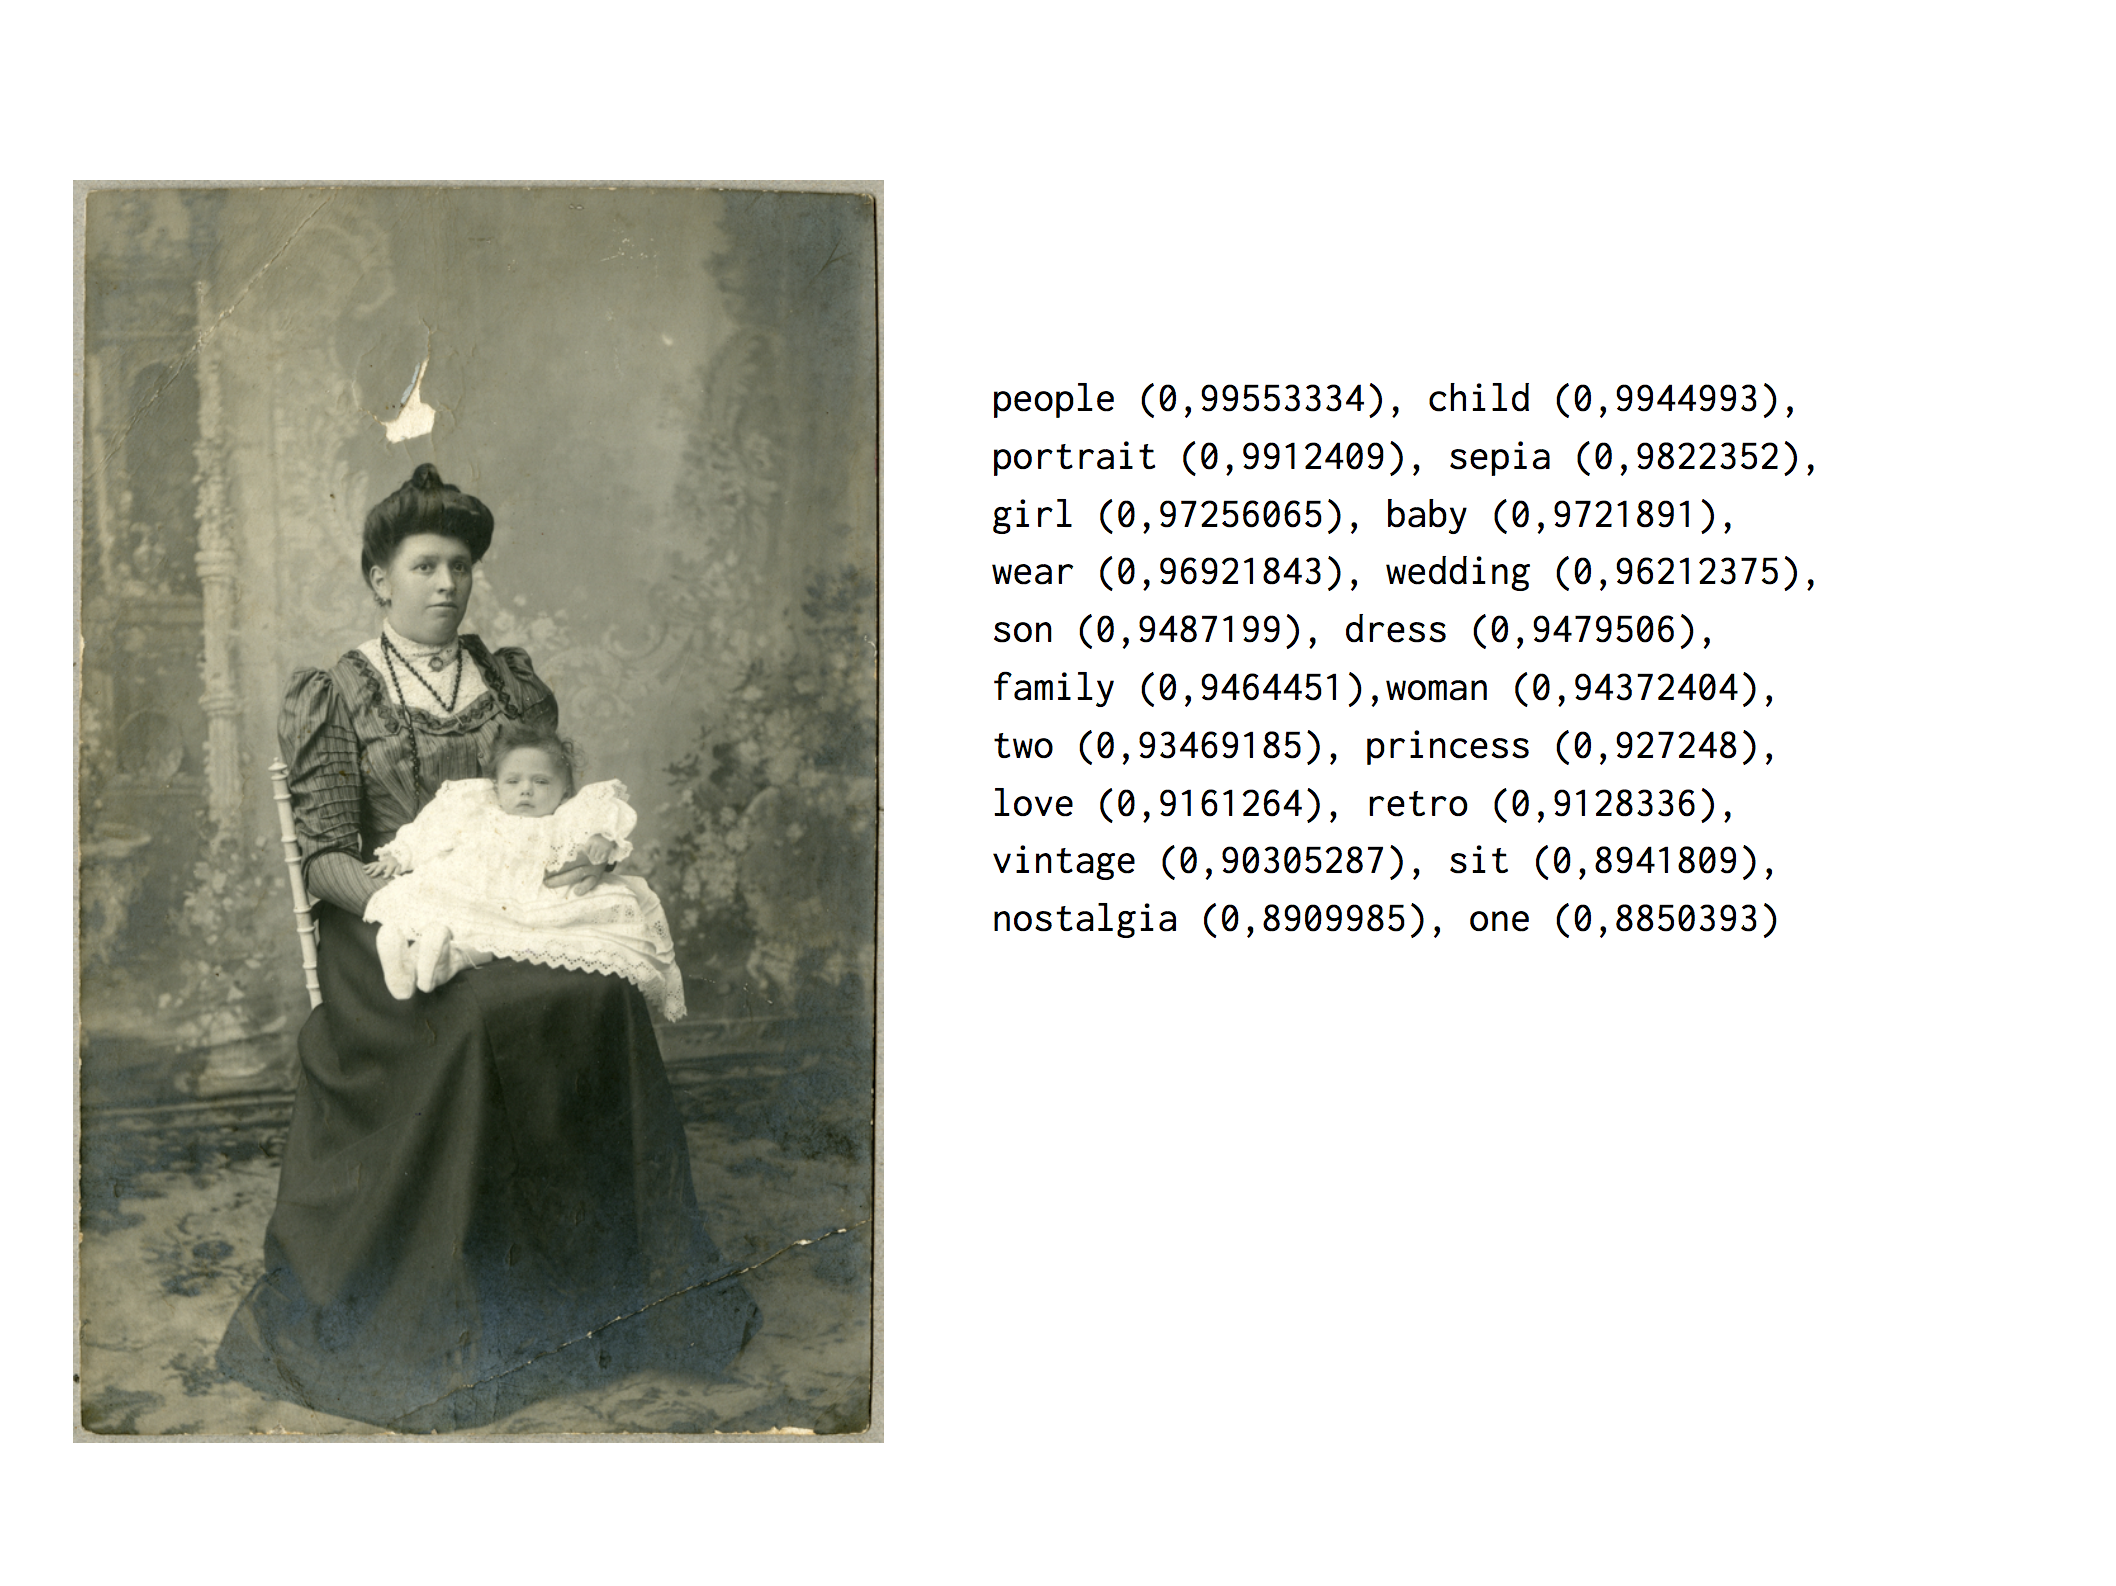
\includegraphics[width=1.0\linewidth]{clarifai}
    \captionof{figure}{\color{HoGentAccent5} Kan Clarifai gebruikt worden voor het beschrijven van historische foto's? (foto: Collectie Huis van Alijn)}
\end{center}\vspace{1cm}

%----------------------------------------------------------------------------------------
%	INTRODUCTION
%----------------------------------------------------------------------------------------

\color{HoGentAccent1} 
\section*{Introductie}
\color{black}
De Vlaamse musea lijden aan een historische achterstand m.b.t. het registreren van de eigen collectie. De metadata blijven meestal beperkt tot formele en adminstratieve gegevens die nodig zijn voor het beheer van de collectiestukken. Registratie is immers tijdrovend werk dat door domeinexperten gedaan wordt. Voor het beschrijven van inhoudelijke informatie zoals afgebeelde personen of objecten, emoties en sfeer ontbreekt het de musea aan tijd en personeel.

Daarenboven is er een digitalisering aan de gang waarbij steeds meer collectiestukken gedigitaliseerd worden. Ook deze digitale beelden moeten voorzien worden van metadata of tags. Het zoeken of vinden van die digitale beelden is immers moeilijk als je bij de zoekactie geen gebruik kunt maken van trefwoorden. Dit verschilt van digitale tekstbestanden, waarbij op basis van \textit{full text search} bestanden teruggevonden kunnen worden. Ook voor dit werk ontbreekt het de musea aan tijd en mankracht. Het gevolg is dat musea over steeds meer beelden beschikken die niet ontsloten of gebruikt kunnen worden. 

Daarom wensten we in deze bachelorproef te onderzoeken of artificiële intelligentie (AI) de collectiemedewerker kan bijstaan in het beschrijven van de cultureel-erfgoedcollecties. Beeldherkenningssoftware is er de laatste jaren enorm op vooruitgegaan en wordt ook steeds eenvoudiger om te gebruiken. Aan de hand van één gekozen API (Clarifai) werd nagegaan of het ingebouwde model van de service voldoende is voor de beschrijving van de beelden en of de software eenvoudig te trainen is voor andere taken. Er werd ook bestudeerd of de software eenvoudig in gebruik is zodat museummedewerkers zelf de API’s kunnen gebruiken om hun beelden te voorzien van inhoudelijke metadata.

%----------------------------------------------------------------------------------------
%	RESEARCH
%----------------------------------------------------------------------------------------

%\color{Black} % DarkSlateGray color for the rest of the content
\color{HoGentAccent1} 
\section*{Onderzoek}
\color{black}

Huis van Alijn heeft een grote fotocollectie over het dagelijkse leven in België in de 20\textsuperscript{e} eeuw. Om de foto’s te kunnen ontsluiten of te doorzoeken, heeft het museum nood aan metadata die een idee geven van wat er op het beeld staat. Tevens worden de foto’s door het museum ingedeeld in thema’s (bv. Huwelijk, Vakantie en Speelgoed) en periodes (bv. 50s, 60s). Het zou een enorme hulp zijn als via beeldherkenning de beelden voorzien worden van beschrijvende metadata en ingedeeld in het juiste thema en periode.

Aan Huis van Alijn werd voorgesteld om volgende use cases te onderzoeken:
\begin{enumerate}
    \item Het automatisch metadateren van iedere foto door het ingebouwde model van de CV API. Voor iedere foto werd de API aangeroepen met het \textit{general}-model van Clarifai. Dit is het meest uigebreide model. Deze metadata werden tevens vergeleken met de bestaande beschrijvingen van de museumregistratoren.
    \item Het classificeren van de foto’s in de thema’s die door Huis van Alijn bepaald werden. Hiervoor werd een \textit{custom} model gecreëerd en werd de CV API getraind. We gingen ook na of het mogelijk is om die classificatie te doen op basis van de tags uit het ingebouwde model van de CV API. 
    \item Het indelen van de foto’s in het decennium waarin ze gemaakt werden. Ook hiervoor werd een custom model ontwikkeld en werd de CV API getraind.
\end{enumerate}

\begin{center}\vspace{1cm}
	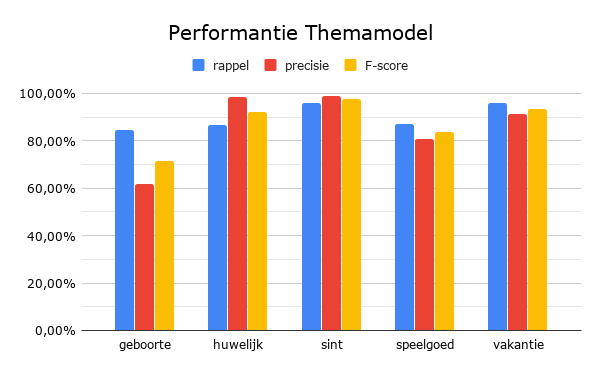
\includegraphics[width=1.0\linewidth]{performantie_themamodel}
	\captionof{figure}{\color{HoGentAccent5} Kan Clarifai gebruikt worden om historische beelden in te delen volgens thema?}
\end{center}\vspace{1cm}

%----------------------------------------------------------------------------------------
%	CONCLUSION
%----------------------------------------------------------------------------------------

\color{HoGentAccent1} 
\section*{Conclusies}
\color{black}
Clarifai bleek erg geschikt te zijn om twee van de drie use cases van Huis van Alijn uit te voeren. Ongeveer 70\% van de tags die het ingebouwde model van Clarifai aanleverde, waren correct. De CV API scoorde vooral goed op universele thema's, zoals geboorte, huwelijk en vakantie. We merkten dat ook heel andere termen gegeven werden dan gangbaar zijn in de registratiepraktijk, zoals tags die de sfeer, emoties en kleur van de foto's beschrijven. Bij foto's van lokale tradities, zoals Sinterklaas, werd ervaren dat het model in de VS gemaakt was. Hierop scoorde de CV API ondermaats. 

Voor het classificeren van de foto’s per thema volstond het ingebouwde model niet. Het zelfgemaakte Themamodel dat de foto's moest indelen volgens thema bleek hiervoor wel erg performant (bijna 90\% correctheid). Hier scoorde de CV API goed op foto's die een vaste weergave hebben, zoals de Sinterklaasfoto's. 

Voor het indelen van de foto's volgens decennium was de trainingset te beperkt. Een pijnpunt tijdens het trainen was immers de kleine en ongelijke dataset. Dat is echter een gangbaar fenomeen in erfgoedcollecties. Verder onderzoek is nodig. 

Om het aantal fouten te vermijden werd voorgesteld om een drempelwaarde in te stellen op de waarschijnlijkheidsscore die door de CV API aan de tags gegeven werd. Bij een te lage score wordt een tag dan niet aanvaard.

%----------------------------------------------------------------------------------------
%	FORTHCOMING RESEARCH
%----------------------------------------------------------------------------------------

\color{HoGentAccent1} 
\section*{Toekomstig onderzoek}
\color{black}

CV API zijn geschikt om de case van Huis van Alijn uit te voeren. Het is op basis van dit onderzoek echter niet mogelijk om te concluderen dat Computer Vision API's gebruikt kunnen worden voor alle soorten cultureel-erfgoedcollecties.  Dit kan verder onderzocht worden met beelden van andere soorten erfgoedmateriaal, denk aan schilderijen, beeldhouwwerken en museumobjecten.

Ook is er onderzoek mogelijk naar andere soorten use cases, zoals pre-iconografische en iconografische beschrijving, gezichtsherkenning, objectregistratie en topic detection.

%----------------------------------------------------------------------------------------

\end{multicols}
\end{document}